% Digital Logic Report Template
% Created: 2020-01-10, John Miller

%==========================================================
%=========== Document Setup  ==============================

% Formatting defined by class file
\documentclass[11pt]{article}

% ---- Document formatting ----
\usepackage[margin=1in]{geometry}	% Narrower margins
\usepackage{booktabs}				% Nice formatting of tables
\usepackage{graphicx}				% Ability to include graphics

%\setlength\parindent{0pt}	% Do not indent first line of paragraphs 
\usepackage[parfill]{parskip}		% Line space b/w paragraphs
%	parfill option prevents last line of pgrph from being fully justified

% Parskip package adds too much space around titles, fix with this
\RequirePackage{titlesec}
\titlespacing\section{0pt}{8pt plus 4pt minus 2pt}{3pt plus 2pt minus 2pt}
\titlespacing\subsection{0pt}{4pt plus 4pt minus 2pt}{-2pt plus 2pt minus 2pt}
\titlespacing\subsubsection{0pt}{2pt plus 4pt minus 2pt}{-6pt plus 2pt minus 2pt}

% ---- Hyperlinks ----
\usepackage[colorlinks=true,urlcolor=blue]{hyperref}	% For URL's. Automatically links internal references.

% ---- Code listings ----
\usepackage{listings} 					% Nice code layout and inclusion
\usepackage[usenames,dvipsnames]{xcolor}	% Colors (needs to be defined before using colors)

% Define custom colors for listings
\definecolor{listinggray}{gray}{0.98}		% Listings background color
\definecolor{rulegray}{gray}{0.7}			% Listings rule/frame color

% Style for Verilog
\lstdefinestyle{Verilog}{
	language=Verilog,					% Verilog
	backgroundcolor=\color{listinggray},	% light gray background
	rulecolor=\color{blue}, 			% blue frame lines
	frame=tb,							% lines above & below
	linewidth=\columnwidth, 			% set line width
	basicstyle=\small\ttfamily,	% basic font style that is used for the code	
	breaklines=true, 					% allow breaking across columns/pages
	tabsize=3,							% set tab size
	commentstyle=\color{gray},	% comments in italic 
	stringstyle=\upshape,				% strings are printed in normal font
	showspaces=false,					% don't underscore spaces
}

% How to use: \Verilog[listing_options]{file}
\newcommand{\Verilog}[2][]{%
	\lstinputlisting[style=Verilog,#1]{#2}
}




%======================================================
%=========== Body  ====================================
\begin{document}

\title{ELC 2137 Lab 1: GitHub and LaTeX Introduction}
\author{Samuel Baker}

\maketitle


\section*{Summary}

In this lab, I attempted to familiarize myself with LaTeX and Github. I did this by first creating my own repository on GitHub and using a LaTeX template in order to create my report for this lab. In the report, I recreated a figure and included Verilog code given to me in my own LaTeX document. All of these changes and modified files were then uploaded to a GitHub repository. At the end of the lab, I had become familiar with both GitHub and the basics of using LaTeX.


\section*{Q\&A}

\begin{enumerate}
	\item What is your GitHub username?
	
	My GitHub username is sg\_baker.
	
	\item What LaTeX enviorment produces a bulleted (non-numbered) list?
	
	The LaTeX enviorment that produces a bulleted list is the \texttt{itemize} enviorment.
	
	\item Write the equation y(t) = 1/2 * e$^t$ using LaTeX equation formatting.
	
	\begin{equation}
		y(t) = \frac{1}{2}e^t
	\end{equation}
	
	\item What is the shortcut key for compiling your LaTeX document?
	
	The shortcut key is F6 to compile.
\end{enumerate}


\section*{Results}

First, I was asked to recreate the figure as shown in Figure 1. I did this by creating a table and a PNG file together in one figure in LaTeX. Then, I was asked to commit this change to the GitHub repository for this lab. The result of that can be seen in Figure 2. Both of these figures are "floating" and were therefore moved to page 3 of the report by LaTeX. I kept both of these figures together by including them inside the same figure enviorment in LaTeX. These results show that I have become familiar with both GitHub's use of local and remote repositories, LaTeX's conventions as a mark-up langauge, and how to properly use said conventions in order to achieve a desired look for a document.

\begin{figure}[ht]\centering
	\begin{tabular}{c|c|c}
		\toprule Binary & Hex & Decimal \\
		\midrule
		0000 & 0 & 0 \\
		0010 & 2 & 2 \\
		0100 & 4 & 4 \\
		0110 & 6 & 6 \\
		1000 & 8 & 8 \\
		1010 & A & 10\\
		\bottomrule
	\end{tabular}\medskip

	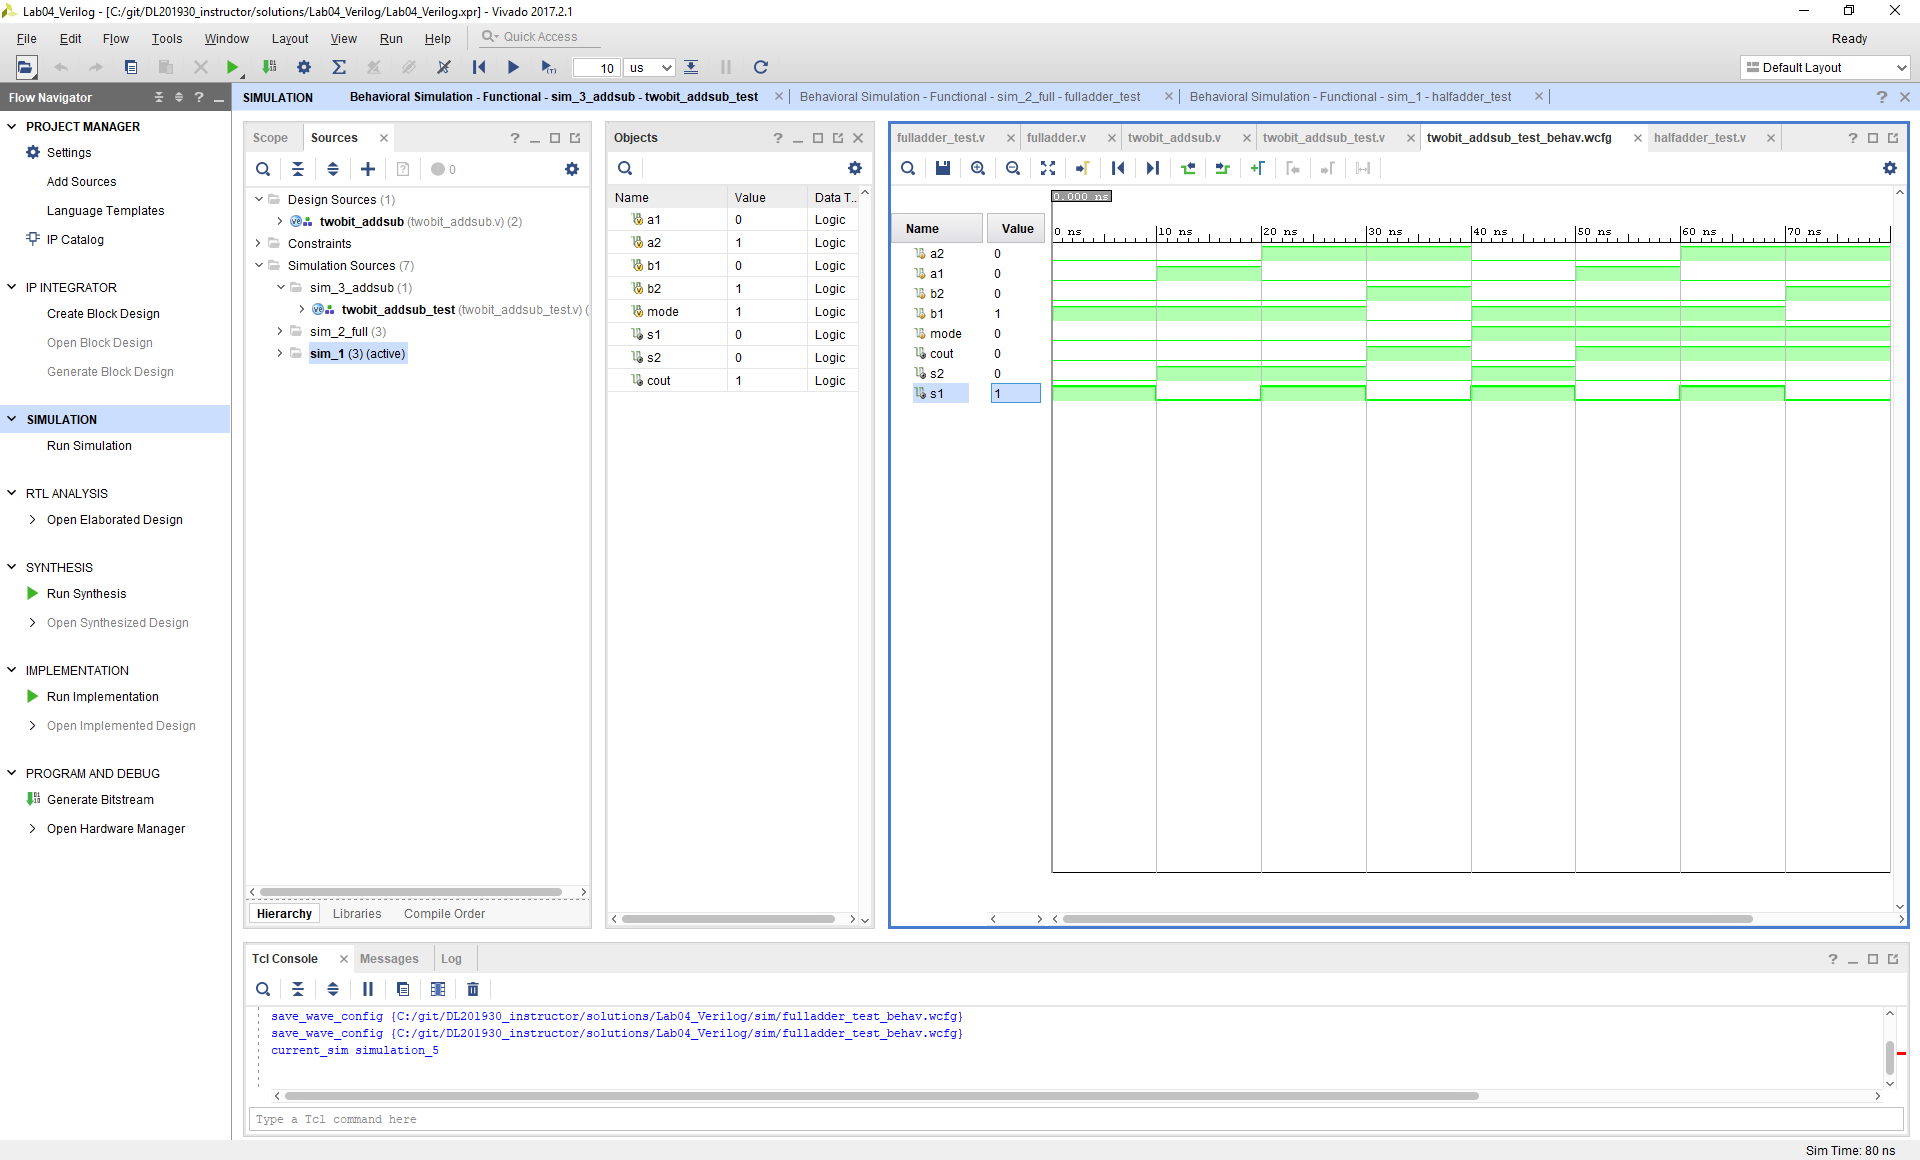
\includegraphics[width=1\textwidth, trim=18.5cm 15.5cm 0.55cm 4.5cm, clip]{lab1_example_screenshot.PNG}
	\caption{Table and simulation waveform to reproduce}
	
	\includegraphics[width=1\textwidth]{github_screenshot.PNG}
	\caption{Screenshot of changes made to GitHub repository}
\end{figure}


\section*{Code}

Below is the example code that was given on canvas. I placed it on the document by using LaTeX's "Listings" package in order to display Verilog code properly.

\Verilog[caption=Example Code from Canvas]{lab1_example_code.sv}

\end{document}
